\chapter{Introduzione}
\label{chap:intro}
\vspace{1cm}
L'obiettivo di questo capitolo è fornire al lettore un'introduzione agli argomenti 
trattati nel corso della tesi, oltre alle motivazioni e a una panoramica del contesto in 
cui si inquadra questo lavoro.

La Sezione \ref{sec:reconfComp} contiene una descrizione dell'area generale in cui si 
svolge il lavoro, presentando i concetti fondamentali alla base del \emph{reconfigurable 
computing}.

La Sezione \ref{sec:definizioneProblema} descrive quindi la problematica dello 
\emph{scheduling}, oggetto del lavoro, alla luce di quanto descritto nella sezione 
precedente.


\section{Reconfigurable computing}
\label{sec:reconfComp}
Oggigiorno, grazie al progresso tecnologico e alla costante riduzione della dimensione 
dei transistor, è resa possibile l'integrazione di diversi componenti elettronici su un 
singolo chip; questi sistemi, chiamati \ac{SoC} o \ac{MPSoC}, a seconda 
che il microprocessore abbia uno o più core, comprendono oltre al processore anche vari 
moduli funzionali quali blocchi di memoria, connettori per interfacce (USB, FireWire, 
Ethernet ecc.) e altre periferiche, collegati tramite BUS.

Questa integrazione tuttavia apre una serie di problemi, tra cui elevato costo di 
progettazione dei sistemi, bassa affidabilità e necessità di controllare il consumo di 
energia; i problemi sopra citati possono essere risolti grazie all'impiego del 
\emph{reconfigurable computing}.

Con il termine \emph{reconfigurable computing} si intende un'architettura hardware che 
offre la possibilità di essere riconfigurata per implementare qualsiasi logica l'utente 
desideri. Le caratteristiche e il fondamento logico alla base di questo tipo di 
architetture sono descritte nelle prossime sezioni.

\subsection{Da von Neumann alle architetture riconfigurabili}
\label{subsec:cambioParadigma}
In questa sezione vengono illustrati i due principali modelli concettuali di architettura
informatica convenzionalmente trattati: il modello \emph{general-purpose} e il modello
\emph{application-specific}. Vengono presentati pregi e difetti di ciascuna architettura
e viene spiegato come il reconfigurable computing cerca di combinare i vantaggi di
entrambe.

\subsubsection{Il modello general-purpose}
Il modello general-purpose è tuttora ampiamente utilizzato, soprattutto nei personal
computer che utilizziamo tutti i giorni. Questa architettura, proposta dal matematico
John von Neumann nel 1945 \cite{First-Draft-Report-EDVAC}, è basata sul concetto di
\emph{stored-program} computer; la particolarità di uno stored-program computer è quella
di tenere le istruzioni dei programmi e i relativi dati nella memoria RAM. Un computer di
questo tipo contiene una \ac{ISA} e può memorizzare un programma composto da un insieme
di queste istruzioni che guideranno la computazione. Contrariamente alle architetture
precedenti, che potevano eseguire solamente un programma preimpostato, il vantaggio
dell'architettura general-purpose consiste nella possibilità di eseguire codice
arbitrario.

\subsubsection{Il modello application-specific}
Mentre il modello visto nella sezione precedente consente di avere una maggiore
flessibilità a discapito però delle prestazioni che può fornire, il modello
application-specific si posiziona all'estremo opposto rispetto al primo: è infatti
caratterizzato da elevate prestazioni e da un basso consumo di potenza. Questo modello
computazionale viene realizzato mediante l'impiego di \ac{ASIC}, dei circuiti integrati
progettati per svolgere un'unica funzionalità. Questo guadagno in prestazioni comporta
uno svantaggio in termini di costi di produzione e naturalmente una minore flessibilità.

Nella prossima sezione viene spiegato come il reconfigurable computing cerca di combinare
i vantaggi di entrambi gli approcci.

\subsubsection{In medio stat virtus}
Secondo l'informatico Reiner Hartenstein, le architetture riconfigurabili introducono un
cambio di paradigma rispetto all'architettura di von Neumann
\cite{HartensteinParadigmShift}. In un articolo del 1991, Hartenstein et al.~presentano
una nuova metodologia di design per lo sviluppo rapido di \ac{ASIC} ad alte prestazioni
partendo da specifiche di algoritmi ad alto livello \cite{HartensteinNovelASICDesign};
questa metodologia è basata su un nuovo paradigma di macchina sequenziale, chiamata da
Hartenstein \emph{anti macchina}\footnote{Così definita per le sue differenze rispetto al
più convenzionale modello di von Neumann.} o \emph{Xputer}\footnote{Il termine
\emph{Xputer} ha origine dalla necessità dei suoi ideatori di rimpiazzare le prime tre
lettere della parola ``computer'' con un altro prefisso. Non trovandone uno, è stato
deciso che queste lettere fossero rimpiazzate dalla lettera ``x''.}.

La principale caratteristica che la differenzia rispetto all'architettura di von Neumann è
l'essere guidata da flussi di dati (data-streams) piuttosto che da flussi di istruzioni
(instruction-streams), idea alla base degli \emph{array sistolici}\footnote{Negli array
sistolici la computazione è affidata a una matrice di \acp{DPU} invece che a \acsp{CPU}
(dalle quali si differenziano per la mancanza di un program counter). La computazione
avviene tramite il trasporto dei dati, che vengono scritti nelle \emph{triggering ports}
delle \acp{DPU}.}.

\begin{table}[ht]
\caption{Classificazione dei paradigmi secondo Nick Tredennick.}
\label{tab:TredennickClassificationScheme}
 \begin{tabular}{l | l}
 \hline
 \textbf{Historic computers} & \textbf{Programming source}\\
 \hline
 resources fixed & none\\
 algorithms fixed & none\\
 \hline
 \textbf{von Neumann computers} & \textbf{Programming source}\\
 \hline
 resources fixed & none\\
 algorithms variable & software (instruction streams)\\
 \hline
 \textbf{Reconfigurable computing} & \textbf{Programming source}\\
 \hline
 resources variable & configware\\
 algorithms variable (anti machine) & flowware (data streams)
 \end{tabular}
\end{table}

Le differenze tra il paradigma del reconfigurable computing e gli altri paradigmi di
computazione sono illustrati da Nick Tredennick nella Tabella
\ref{tab:TredennickClassificationScheme} \cite{TredennickClassification}: si può
osservare che le architetture riconfigurabili offrono la possibilità di configurare sia le
risorse per la computazione (\emph{configware}) sia gli algoritmi da eseguire
(\emph{flowware}). Tale soluzione porta a un minore costo di progettazione e
maggiore flessibilità rispetto a circuiti dedicati e a prestazioni superiori rispetto a
soluzioni general-purpose.

Viene ora illustrata la struttura generica di un'architettura riconfigurabile.

\subsubsection{I dispositivi riconfigurabili}
Le architetture riconfigurabili sono composte da un processore general-purpose e da una
porzione di logica riconfigurabile: lo scopo del processore è controllare le
attività (d'ora in avanti definite \emph{task}) in esecuzione sulla logica
riconfigurabile e di gestire le comunicazioni da e verso l'esterno. Le informazioni per la
(ri)configurazione che devono essere ``caricate'' sul dispositivo sono contenute in un
file chiamato \emph{bitstream}.

Esempi molto diffusi di dispositivi riconfigurabili sono le schede \emph{\acp{FPGA}},
introdotte attorno alla metà degli anni '80, che contengono sia logica che comunicazioni
programmabili. La logica può essere configurata per rappresentare delle porte logiche
oppure per sintetizzare dei core \ac{IP}.

Inizialmente, il reconfigurable computing veniva utilizzato per realizzare prototipi
economici di soluzioni hardware. Continui progressi tecnologici hanno portato
a un'evoluzione della fase di riconfigurazione, qui descritta:
\begin{enumerate}
 \item \emph{Riconfigurazione a Compile Time}: il dispositivo è configurato soltanto
dopo la fase di design, prima dell'esecuzione dell'applicazione;
 \item \emph{Riconfigurazione a Run Time}: il dispositivo può essere riconfigurato
interrompendo temporaneamente l'esecuzione dell'applicazione;
 \item \emph{Riconfigurazione Parziale Dinamica}, in inglese \ac{PDR}: parte della logica
può essere riconfigurata tramite un bitstream parziale, senza interrompere i task in
esecuzione su altre regioni del dispositivo.
\end{enumerate}

% TODO: applicazioni del reconfigurable computing?

Nella prossima sezione vengono descritte le motivazioni e la problematica oggetto del
lavoro.

\section{Definizione del problema}
\label{sec:definizioneProblema}
Le prossime sezioni illustreranno uno dei campi di applicazione delle architetture
riconfigurabili, con le relative problematiche che emergono.

\subsection{Hardware/Software Co-design}
Come visto nella precedente sezione, il reconfigurable computing offre elevate
prestazioni senza sacrificare la flessibilità, e rappresenta un'area di
ricerca in continua crescita. Per questo motivo, date anche la crescente complessità
delle applicazioni e la richiesta di elevate prestazioni, i sistemi embedded
eterogenei\footnote{I sistemi embedded eterogenei sono dispositivi progettati per
svolgere un numero limitato di funzioni con requisiti di alte prestazioni, basso consumo
energetico e prestazioni in tempo reale, come i normali sistemi embedded; si
differenziano da questi perchè parte dell'applicazione può essere eseguita da
acceleratori hardware (ad esempio una porzione di scheda riconfigurabile FPGA), da
hardware general-purpose oppure da \acp{DSP}.} stanno guadagnando popolarità.

Il nuovo paradigma introdotto dalle architetture riconfigurabili procura vantaggi
soprattutto nel design \ac{ESL}, in particolare l'\mbox{hardware/software} co-design.
Prima delle architetture riconfigurabili, le due parti (hardware e software) erano
sviluppate separatamente e integrate successivamente; la ricerca su 
\mbox{hardware/software} co-design invece ha come obiettivo la creazione di strumenti che 
permettano lo sviluppo contemporaneo delle due componenti, con possibilità di esplorare e 
analizzare trade-off durante il design del sistema. In questo modo si permette al 
designer di concentrarsi sullo sviluppo dell'applicazione ad alto livello, parzialmente 
astraendo dal livello più basso (ad esempio generazione dei core che implementano i vari 
task, oppure delle direttive di sincronizzazione).

Il flusso di design automatizzato dovrebbe consentire la realizzazione della sintesi ad 
alto livello (\emph{high-level synthesis}): partendo da un'applicazione scritta in un
linguaggio ad alto livello, opportunamente annotata per istruire il tool sui vari task
da eseguire, e da una descrizione dell'architettura riconfigurabile, il tool deve gestire
le seguenti fasi:
\begin{enumerate}
 \item \emph{Mapping}: decisione di quale task deve essere eseguito su quale processing 
element  (\mbox{hardware/software} partitioning) e, nel caso di più implementazioni per 
ogni task, quale implementazione eseguire;
 \item \emph{Scheduling}: assegnazione dei tempi di inizio/fine esecuzione dei task;
 \item \emph{Floorplacement} o \emph{floorplanning}: in questa fase si identificano i 
task che idealmente dovrebbero essere posti fisicamente ``vicini'' sulla scheda, ad 
esempio per minimizzare la latenza della comunicazione, rispettando i vincoli di area 
riconfigurabile a disposizione.
\end{enumerate}

Il lavoro descritto in questa tesi si concentra su una possibile soluzione per il 
problema di scheduling dei task, che verrà spiegato più in dettaglio nella prossima 
sezione.


\subsection{La fase di scheduling}
L'obiettivo dello scheduler è assegnare i tempi di inizio e di fine dell'esecuzione ai
task che compongono l'applicazione.

\begin{figure}[ht]
 \begin{center}
 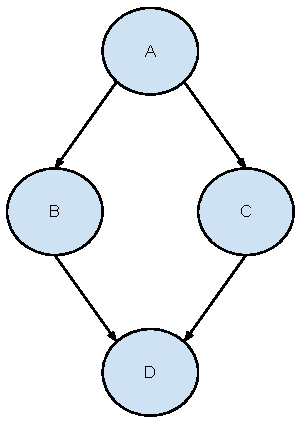
\includegraphics[width=0.7\textwidth]{./capitoli/figure/TaskGraphExample.pdf}
 \caption{Esempio di task graph.}
 \label{fig:taskGraphExample}
 \end{center}
\end{figure}

Lo scheduler riceve i dati relativi all'applicazione sotto forma di ``task graph''.
In Figura \ref{fig:taskGraphExample} è raffigurato un esempio di task graph: esso è un 
grafo orientato aciclico\footnote{\ac{DAG}.} in cui i nodi rappresentano i vari task da 
eseguire, e gli archi rappresentano le precedenze tra questi task.
Le precedenze esplicitano relazioni produttore-consumatore, ovvero un arco orientato 
$(i,j)$ simboleggia un trasferimento dell'output della computazione del task $i$ in 
memoria (locale o condivisa), per essere utilizzato successivamente come input per il 
task $j$; gli archi introducono quindi delle comunicazioni che devono necessariamente 
essere prese in considerazione nella fase di scheduling.

Oltre alle comunicazioni, lo scheduler deve anche gestire il verificarsi di 
riconfigurazioni nel corso dell'esecuzione dell'applicazione. Ad esempio, se due task $i$ 
e $j$ durante la fase di mapping vengono assegnati a uno stesso processing element su 
scheda con due implementazioni diverse, è necessario riconfigurare quella porzione di 
scheda dopo l'esecuzione di $i$ e prima dell'esecuzione di $j$.


\subsubsection{Complessità del problema}
Il problema di fissare uno schedule per i task di un'applicazione è un classico esempio 
di \ac{RCSP}; tale problema appartiene alla classe di complessità computazionale 
NP-hard.

% (si veda l'Appendice \ref{chap:appA} per un riepilogo delle classi di 
% complessità computazionale).

% l'aumento di risorse logiche
% configurabili e delle possibilità di utilizzo di tali risorse, unito alle innovazioni
% tecnologiche quali ad esempio la \ac{PDR} hanno portato alla necessità di sviluppare
% strumenti per il \ac{CAD} sempre più complessi. Questi strumenti guidano i designer in
% fase di progettazione e implementazione di un sistema riconfigurabile, nei seguenti
% compiti:
% \begin{itemize}
%  \item Analisi per il design dell'architettura riconfigurabile da utilizzare;
%  \item Sintesi delle applicazioni/attività in hardware;
%  \item Simulazione dell'esecuzione del programma per verificare il comportamento
% dell'hardware;
%  \item Piazzamento dei task e ``instradamento'' delle comunicazioni tra i vari blocchi
% funzionali.
% \end{itemize}
% 
% Un esempio di tool \ac{CAD} è l'\ac{EDK} sviluppato da Xilinx \cite{XilinxEDK}, che
% integra sia i componenti software che hardware visti precedentemente.

